\chapter{EKSPERIMEN DAN HASIL}
\label{chap:pengujiananalisis}

% Ubah bagian-bagian berikut dengan isi dari pengujian dan analisis

Pada penelitian ini dipaparkan hasil pengujian serta analisis dari desain sistem dan implementasi. Penggunaan dataset dari PKU Sketch Re-ID telah diambil dan telah meminta izin kepada \textit{National Engineering Laboratory for Video Technology}, Universitas Peking.
Pengujian ini dilakukan dalam empat bagian, yakni sebagai berikut:

\begin{enumerate}[nolistsep]
	\item Pengujian menggunakan Lightweight Residual Network
	\item Pengujian menggunakan Lightweight Residual Network \textit{pre-trained} pada Market-1501
	\item Pengujian menggunakan Re-Ranking
	\item Studi Ablasi
	\item Pengujian dengan menggunakan Ensemble.
	
	\vspace{1ex}
\end{enumerate}

Pada pengujian ini, pelatihan masing-masing model dilakukan dengan menggunakan laptop dengan spesifikasi \textit{hardware} sebagai berikut:

\begin{table}[h!]
	\begin{center}
		\begin{tabular}{|c|c|}
			\hline
			\textbf{Processor} & Intel(R) Core(TM) i7-8750H CPU @ 2.20GHz \\ \hline
			\textbf{RAM} & 8 GB DIMM DDR4 x 2\\ \hline
			\textbf{Storage} & HDD 512 GB \\ \hline
			\textbf{Graphics Card} & Nvidia GeForce GTX 1060 6GB MAX-Q \\ \hline
			\textbf{Operating System} & Ubuntu 18.04 LTS 64-bit \\ \hline
		\end{tabular}
	\end{center}
	\vspace{1ex}
	\caption{Spesifikasi Laptop yang digunakan}
	\label{tabel:3}
\end{table}


\section{Pengujian menggunakan Lightweight Residual Network}
\label{sec: nopretrained}
\vspace{1ex}
Pada pengujian ini, dilakukan \textit{training} dengan menggunakan Lightweight Residual Network, dimana pada model tidak dilakukan pelatihan ke dataset Market-1501 sebelum dilatih untuk melakukan klasifikasi pada dataset PKU Sketch Re-ID. Selain itu pada tahap pengujian ini dilakukan dua metode pengujian, yaitu dengan menggunakan metode Local Binary Pattern dan metode CycleGAN untuk menjembatani modalitas antara citra sketsa dan citra CCTV. Pada tahap pengujian ini hanya dilakukan pengujian pada model ResNet 20, pengujian seperti ini dilakukan karena model ini membutuhkan waktu \textit{training} paling sedikit dibandingkan dengan model \textit{lightweight} ResNet lain yang akan digunakan pada pengujian selanjutnya.

Tabel \ref{tabel: 4} menunjukan hasil dari training dan testing model sebanyak 10 kali untuk model ResNet 20 tanpa adanya perubahan pada dataset PKU Sketch Re-ID.

\vspace{1ex}

\begin{longtable}{|c|c|c|c|c|}
	\caption{Rata-rata performa ResNet 20}
	\label{tabel: 4}\\
	\hline
	\rowcolor[HTML]{C0C0C0}
	\textbf{No} &\textbf{Rank-1} & \textbf{Rank-5} & \textbf{Rank-10} & \textbf{mAP} \\
	\hline
	1 & 8 & 32 & 48 & 11.4505\\
	2 & 10 & 32 & 46 & 11.2543\\
	3 & 4 & 32 & 46 & 8.426\\
	4 & 8 & 24 & 32 & 9.842\\
	5 & 8 & 36 & 48 & 11.1407\\
	6 & 10 & 28 & 42 & 11.7093\\
	7 & 6 & 32 & 50 & 9.9849\\
	8 & 10 & 28 & 44 & 10.8898\\
	9 & 14 & 26 & 44 & 14.43\\
	10 & 8 & 26 & 42 & 10.3942\\
	\hline
	\textbf{Average} & 8.6 & 29.6 & 44.2 & 10.95217\\
	\hline
\end{longtable}

\vspace{1ex}

\subsection{\textit{Local Binary Pattern} (LBP)}

Tabel \ref{tabel: 5} menunjukan hasil dari training dan testing model sebanyak 10 kali untuk model ResNet 20 dengan menggunakan \textit{filter} LBP. Namun dikarenakan hasil yang didapatkan lebih rendah dibandingkan tanpa menggunakan LBP pada semua metrik evaluasi, sedangkan waktu yang dibutuhkan untuk \textit{training} menjadi 2 kali lebih banyak pengujian menggunakan LBP diberhentikan.

\begin{longtable}{|c|c|c|c|c|}
	\caption{Rata-rata performa ResNet 20 dengan Local Binary Pattern}
	\label{tabel: 5}\\
	\hline
	\rowcolor[HTML]{C0C0C0}
	\textbf{No} &\textbf{Rank-1} & \textbf{Rank-5} & \textbf{Rank-10} & \textbf{mAP} \\
	\hline
	1 & 2 & 30 & 40 & 7.7963\\
	2 & 4 & 26 & 44 & 8.898\\
	3 & 6 & 32 & 46 & 10.3007\\
	4 & 12 & 30 & 42 & 13.5232\\
	5 & 14 & 24 & 40 & 12.4012\\
	6 & 8 & 24 & 38 & 10.4669\\
	7 & 8 & 32 & 42 & 11.4641\\
	8 & 4 & 30 & 44 & 9.9319\\
	9 & 8 & 28 & 38 & 10.0783\\
	10 & 10 & 14 & 30 & 9.7921\\
	\hline
	\textbf{Average} & 7.6 & 27 & 40.4 & 10.46527\\
	\hline
\end{longtable}

\subsection{CycleGAN}

Tabel \ref{tabel: 6} menunjukan hasil dari training dan testing model sebanyak 10 kali untuk model ResNet 20 dimana citra sketsa pada dataset PKU Sketch Re-Identification telah dilakukan translasi \textit{style}.

\begin{longtable}{|c|c|c|c|c|}
	\caption{Rata-rata performa ResNet 20 dengan CycleGAN}
	\label{tabel: 6}\\
	\hline
	\rowcolor[HTML]{C0C0C0}
	\textbf{No} &\textbf{Rank-1} & \textbf{Rank-5} & \textbf{Rank-10} & \textbf{mAP} \\
	\hline
	1 & 8 & 16 & 34 & 8.9563\\
	2 & 12 & 28 & 36 & 14.2855\\
	3 & 10 & 24 & 40 & 10.558\\
	4 & 8 & 26 & 36 & 10.4396\\
	5 & 8 & 22 & 40 & 10.8883\\
	6 & 10 & 26 & 44 & 10.9954\\
	7 & 6 & 34 & 50 & 9.7\\
	8 & 14 & 28 & 42 & 13.4316\\
	9 & 8 & 26 & 42 & 10.5551\\
	10 & 10 & 26 & 38 & 12.737\\
	\hline
	\textbf{Average} & 9.4 & 25.6 & 40.2 & 11.25468\\
	\hline
\end{longtable}

Meskipun Rank-5 dan Rank-10 yang didapatkan lebih rendah, dikarenakan metrik evaluasi yang digunakan disamakan dengan pada paper "Cross-Domain Adversarial Feature Learning for Sketch Re-identification", yaitu menggunakan Rank-1 accuracy. Maka semua pengujian selanjutnya akan dilakukan menggunakan dataset yang telah ditranslasi dengan CycleGAN.

\section{Pengujian menggunakan Lightweight Residual Network \textit{pre-trained} pada Market-1501}
\label{sec:pretrained}

Pada pengujian ini dilakukan \textit{pre-training} terlebih dahulu pada dataset Market 1501 untuk mengatasi keterbatasan data pada dataset PKU Sketch Re-ID. Pada tahap pengujian ini, digunakan tiga jenis \textit{Lightweight Residual Network} yakni; ResNet 20, ResNet 56, dan ResNet 110. Dataset yang digunakan pada tahap pengujian ini semuanya merupakan hasil sintesis dari CycleGAN. 

\subsection{ResNet 20}

Tabel \ref{tabel: 7} menunjukan hasil dari training dan testing model sebanyak 10 kali untuk model ResNet 20 dengan model yang telah di \textit{pre-trained} pada dataset Market 1501 terlebih dahulu.

\vspace{1ex}

\begin{longtable}{|c|c|c|c|c|}
	\caption{Rata-rata performa ResNet 20 \textit{pretrained} pada Market 1501 }
	\label{tabel: 7}\\
	\hline
	\rowcolor[HTML]{C0C0C0}
	\textbf{No} &\textbf{Rank-1} & \textbf{Rank-5} & \textbf{Rank-10} & \textbf{mAP} \\
	\hline
	1 & 12 & 28 & 42 & 11.6169\\
	2 & 8 & 24 & 40 & 10.1131\\
	3 & 10 & 30 & 46 & 12.5311\\
	4 & 10 & 24 & 32 & 10.3256\\
	5 & 10 & 22 & 40 & 9.7441\\
	6 & 10 & 22 & 48 & 10.4837\\
	7 & 10 & 34 & 40 & 13.0863\\
	8 & 14 & 38 & 48 & 13.5198\\
	9 & 8 & 18 & 32 & 9.6554\\
	10 & 10 & 24 & 42 & 10.9248\\
	\hline
	\textbf{Average} & 10.2 & 26.4 & 41 & 11.30008\\
	\hline
\end{longtable}

\vspace{1ex}
Dapat dilihat terdapat peningkatan yang cukup signifikan pada Rank-1 accuracy yaitu dari 9,4\% ke 10,2\%. Selain itu Rank-5, Rank-10 , dan mAP yang didapatkan lebih tinggi dibandingkan pada saat tidak di \textit{pre-trained} pada Market 1501.

\subsection{ResNet56}

Tabel \ref{tabel: 8} menunjukan hasil dari training dan testing model sebanyak 10 kali untuk model ResNet 56 dengan model yang telah di \textit{pre-trained} pada dataset Market 1501 terlebih dahulu.

\vspace{1ex}

\begin{longtable}{|c|c|c|c|c|}
	\caption{Rata-rata performa ResNet 56 \textit{pretrained} pada Market 1501 }
	\label{tabel: 8}\\
	\hline
	\rowcolor[HTML]{C0C0C0}
	\textbf{No} &\textbf{Rank-1} & \textbf{Rank-5} & \textbf{Rank-10} & \textbf{mAP} \\
	\hline
	1 & 20 & 44 & 54 & 19.2315\\
	2 & 16 & 34 & 42 & 20.2117\\
	3 & 14 & 34 & 50 & 17.2698\\
	4 & 16 & 36 & 40 & 16.8498\\
	5 & 10 & 34 & 48 & 14.9505\\
	6 & 12 & 26 & 36 & 14.3816\\
	7 & 14 & 32 & 46 & 14.9699\\
	8 & 12 & 38 & 60 & 16.0066\\
	9 & 10 & 38 & 46 & 14.5599\\
	10 & 18 & 34 & 46 & 19.1052\\
	\hline
	\textbf{Average} & 14.2 & 35 & 47.8 & 16.95365\\
	\hline
\end{longtable}

Terlihat terdapat peningkatan yang sangat signifikan pada Rank-1, yaitu sebesar 40\% apabila dibandingkan dengan ResNet 20.

\subsection{ResNet 110}

Tabel \ref{tabel: 9} menunjukan hasil dari training dan testing model sebanyak 10 kali untuk model ResNet 110 dengan model yang telah di \textit{pre-trained} pada dataset Market 1501 terlebih dahulu. Pada pengujian ini terlihat terdapat peningkatan yang sangat signifikan pada Rank-1, yaitu sebesar 70\% apabila dibandingkan dengan ketika menggunakan model ResNet 20.

\vspace{1ex}

\begin{longtable}{|c|c|c|c|c|}
	\caption{Rata-rata performa ResNet 110 \textit{pretrained} pada Market 1501 }
	\label{tabel: 9}\\
	\hline
	\rowcolor[HTML]{C0C0C0}
	\textbf{No} &\textbf{Rank-1} & \textbf{Rank-5} & \textbf{Rank-10} & \textbf{mAP} \\
	\hline
	1 & 18 & 36 & 56 & 17.9811\\
	2 & 20 & 46 & 62 & 21.6104\\
	3 & 18 & 40 & 56 & 19.7356\\
	4 & 16 & 44 & 54 & 18.3177\\
	5 & 18 & 46 & 56 & 18.1901\\
	6 & 16 & 38 & 42 & 17.9401\\
	7 & 18 & 36 & 54 & 20.0548\\
	8 & 16 & 38 & 52 & 18.2794\\
	9 & 12 & 26 & 38 & 14.3971\\
	10 & 22 & 38 & 52 & 22.2614\\
	\hline
	\textbf{Average} & 17.4 & 38.8 & 52.2 & 18.87587\\
	\hline
\end{longtable}
\vspace{2ex}
\section{Pengujian menggunakan Re-Ranking}
\vspace{2ex}
Pada tahap pengujian ini dilakukan Re-Ranking pada hasil training dan testing 10 kali yang telah dilakukan pada model Residual Network 56 dan 110. Re-Ranking dilakukan dengan harapan dapat meningkatkan performa Rank-1 model, dikarenakan dari penelitian re-identifikasi orang, dapat dilihat bahwa \textit{re-ranking} dapat meningkatkan performa Rank-1 dan mAP model.
\vspace{2ex}
\subsection{Re-Ranking pada ResNet 56}
\vspace{2ex}
Pada tahap pengujian ini dilakukan re-ranking terhadap 10 metrik evaluasi yang tertera pada tabel \ref{tabel: 8}, dimana reranking merupakan pengambilan jarak antara citra query dan citra gallery yang terdekat. Dapat dilihat pada hasil \textit{re-ranking} di tabel \ref{tabel:10}, bahwa semua metrik evaluasi yang digunakan menurun drastis. Yaitu masing-masing sebesar 6.2\% , 9.6\%, 5\%, dan 0.18\%. Hal ini menunjukan bahwa re-identifikasi sketsa merupakan sebuah permasalahan yang sangat berbeda dengan re-identifikasi manusia.

\begin{longtable}{|c|c|c|c|c|}
	\caption{Rata-rata performa ResNet 56 dengan re-ranking}
	\label{tabel:10}\\
	\hline
	\rowcolor[HTML]{C0C0C0}
	\textbf{No} &\textbf{Rank-1} & \textbf{Rank-5} & \textbf{Rank-10} & \textbf{mAP} \\
	\hline
	1 &8 &26 &34 &10.5473 \\
	2 &8 &28 &38 &11.8655 \\
	3 &6 &28 &38 &10.9266 \\
	4 &8 &22 &30 &10.9797 \\
	5 &8 &20 &34 &11.7746 \\
	6 &6 &26 &34 &10.4775 \\
	7 &6 &26 &36 &10.8615 \\
	8 &10 &26 &34 &12.5916 \\
	9 &6 &26 &38 &10.3757 \\
	10 &14 &26 &44 &14.4551 \\
	\hline
	\textbf{Average} & 8 & 25.4 & 36 &11.48551 \\
	\hline
\end{longtable}

\subsection{Re-Ranking pada ResNet 110}
\vspace{2ex}
Sama dengan pada Residual Network 56 dapat dilihat bahwa re-ranking menyebabkan terjadinya penurunan pada semua metrik evaluasi.

\begin{longtable}{|c|c|c|c|c|}
	\caption{Rata-rata performa ResNet 110 dengan re-ranking}
	\label{tabel:11}\\
	\hline
	\rowcolor[HTML]{C0C0C0}
	\textbf{No} &\textbf{Rank-1} & \textbf{Rank-5} & \textbf{Rank-10} & \textbf{mAP} \\
	\hline
	1 &8 &24 &40 &12.0668 \\
	2 &10 &34 &36 &13.4624 \\
	3 &6 &24 &34 &10.1525 \\
	4 &10 &26 &38 &14.866 \\
	5 &16 &32 &46 &17.1341 \\
	6 &10 &20 &26 &12.8491 \\
	7 &14 &30 &36 &16.3645 \\
	8 &18 &30 &42 &19.7371 \\
	9 &6 &22 &36 &9.6301 \\
	10 &8 &24 &38 &10.146 \\
	\hline
	\textbf{Average} & 10.6 & 26.6 & 37.2 &13.640859 \\
	\hline
\end{longtable}

\pagebreak

\subsection{Kesimpulan Re-Ranking untuk Re-Identifikasi Sketsa}
Dari pengujian yang dilakukan pada kedua model, dapat dilihat bahwa \textit{re-ranking} yang dilakukan menyebabkan penurunan performa yang sangat drastis pada kedua model. Selain itu dapat dilihat bahwa pada semua metrik evaluasi, tidak ada yang meningkat, berbeda dengan pada re-identifikasi manusia dimana Rank-1 dan mean Average Precision meningkat. Oleh karena hasil yang kami dapatkan sebagai berikut maka percobaan dengan \textit{re-ranking} tidak akan dilanjutkan lebih lagi. Tabel dibawah menunjukkan perbedaan performa rata-rata dari kedua model dengan hasil re-rankingnya.

\section{Pengujian menggunakan Re-Ranking}
\vspace{2ex}
Pada tahap pengujian ini dilakukan Re-Ranking pada hasil training dan testing 10 kali yang telah dilakukan pada model Residual Network 56 dan 110. Re-Ranking dilakukan dengan harapan dapat meningkatkan performa Rank-1 model, dikarenakan dari penelitian re-identifikasi orang, dapat dilihat bahwa \textit{re-ranking} dapat meningkatkan performa Rank-1 dan mAP model.
\vspace{2ex}
\subsection{Re-Ranking pada ResNet 56}
\vspace{2ex}
Pada tahap pengujian ini dilakukan re-ranking terhadap 10 metrik evaluasi yang tertera pada tabel \ref{tabel: 8}, dimana reranking merupakan pengambilan jarak antara citra query dan citra gallery yang terdekat. Dapat dilihat pada hasil \textit{re-ranking} di tabel \ref{tabel:10}, bahwa semua metrik evaluasi yang digunakan menurun drastis. Yaitu masing-masing sebesar 6.2\% , 9.6\%, 5\%, dan 0.18\%. Hal ini menunjukan bahwa re-identifikasi sketsa merupakan sebuah permasalahan yang sangat berbeda dengan re-identifikasi manusia.

\pagebreak

\begin{longtable}{|c|c|c|c|c|}
	\caption{Rata-rata performa ResNet 56 dengan re-ranking}
	\label{tabel:10}\\
	\hline
	\rowcolor[HTML]{C0C0C0}
	\textbf{No} &\textbf{Rank-1} & \textbf{Rank-5} & \textbf{Rank-10} & \textbf{mAP} \\
	\hline
	1 &8 &26 &34 &10.5473 \\
	2 &8 &28 &38 &11.8655 \\
	3 &6 &28 &38 &10.9266 \\
	4 &8 &22 &30 &10.9797 \\
	5 &8 &20 &34 &11.7746 \\
	6 &6 &26 &34 &10.4775 \\
	7 &6 &26 &36 &10.8615 \\
	8 &10 &26 &34 &12.5916 \\
	9 &6 &26 &38 &10.3757 \\
	10 &14 &26 &44 &14.4551 \\
	\hline
	\textbf{Average} & 8 & 25.4 & 36 &11.48551 \\
	\hline
\end{longtable}

\subsection{Re-Ranking pada ResNet 110}
\vspace{2ex}
Sama dengan pada Residual Network 56 dapat dilihat bahwa re-ranking menyebabkan terjadinya penurunan pada semua metrik evaluasi.

\begin{longtable}{|c|c|c|c|c|}
	\caption{Rata-rata performa ResNet 110 dengan re-ranking}
	\label{tabel:11}\\
	\hline
	\rowcolor[HTML]{C0C0C0}
	\textbf{No} &\textbf{Rank-1} & \textbf{Rank-5} & \textbf{Rank-10} & \textbf{mAP} \\
	\hline
	1 &8 &24 &40 &12.0668 \\
	2 &10 &34 &36 &13.4624 \\
	3 &6 &24 &34 &10.1525 \\
	4 &10 &26 &38 &14.866 \\
	5 &16 &32 &46 &17.1341 \\
	6 &10 &20 &26 &12.8491 \\
	7 &14 &30 &36 &16.3645 \\
	8 &18 &30 &42 &19.7371 \\
	9 &6 &22 &36 &9.6301 \\
	10 &8 &24 &38 &10.146 \\
	\hline
	\textbf{Average} & 10.6 & 26.6 & 37.2 &13.640859 \\
	\hline
\end{longtable}

\pagebreak

\subsection{Kesimpulan Re-Ranking untuk Re-Identifikasi Sketsa}
Dari pengujian yang dilakukan pada kedua model, dapat dilihat bahwa \textit{re-ranking} yang dilakukan menyebabkan penurunan performa yang sangat drastis pada kedua model. Selain itu dapat dilihat bahwa pada semua metrik evaluasi, tidak ada yang meningkat, berbeda dengan pada re-identifikasi manusia dimana Rank-1 dan mean Average Precision meningkat. Oleh karena hasil yang kami dapatkan sebagai berikut maka percobaan dengan \textit{re-ranking} tidak akan dilanjutkan lebih lagi. Tabel dibawah menunjukkan perbedaan performa rata-rata dari kedua model dengan hasil re-rankingnya.

\begin{table}[h!]
	\begin{center}
		\begin{tabular}{|c|c|c|c|c|}
			\hline
			\textbf{Name} & \textbf{Rank-1} & \textbf{Rank-5} & \textbf{Rank-10} & \textbf{mAP} \\ \hline
			ResNet 56 & 14.2\% & 35\% & 47.8\% & 16.95\%\\ \hline
			ResNet 56 + re-rank  & 8\% & 25.4\% & 36\% & 11.49\%\\ \hline
			ResNet 110 & 17.4\% & 38.8\% & 52.2\% & 18.88\%\\ \hline
			ResNet 110 + re-rank & 10.6\% & 26.6\% & 37.2\% & 13.64\%\\ \hline
		\end{tabular}
	\end{center}
\end{table}
\vspace{-3ex}
\section{Studi Ablasi}
\subsection{Perubahan pada Fully Connected Layer}
\vspace{1ex}

Pada tahap pengujian ini dilakukan perubahan \textit{Fully Connected layer} pertama yang terdapat pada ResNet 56 dan ResNet 110. Studi Ablasi hanya dilakukan pada kedua model tersebut dikarenakan terjadi peningkatan yang sangat signifikan dibanding dengan menggunakan ResNet 20, yaitu 40\% dan 70\%. Pengujian ini dilakukan dengan 5 jenis \textit{Fully Connected Layer} yaitu:

\begin{enumerate}[nolistsep]
	\item \textit{Fully Connected} 128
	\item \textit{Fully Connected} 256
	\item \textit{Fully Connected} 512
	\item \textit{Fully Connected} 768
	\item \textit{Fully Connected} 1024
	\vspace{1ex}
\end{enumerate}

Semua pengujian sebelumnya dilakukan dengan \textit{Fully Connected layer} sebesar 512. Oleh karena itu, pada bagian ini dilakukan pengujian pada Fully Connected lainnya yang tertera.

\pagebreak

\subsection{ResNet 56 Fully Connected 128}
\vspace{1ex}
\begin{longtable}{|c|c|c|c|c|}
	\caption{Rata-rata performa ResNet 56 Fully Connected 128 \textit{pretrained} pada Market 1501}
	\label{tabel: 10}\\
	\hline
	\rowcolor[HTML]{C0C0C0}
	\textbf{No} &\textbf{Rank-1} & \textbf{Rank-5} & \textbf{Rank-10} & \textbf{mAP} \\
	\hline
	1 &8 &42 &52 &13.4307 \\
	2 &14 &36 &48 &15.8562 \\
	3 &12 &28 &40 &13.4272 \\
	4 &10 &34 &50 &15.0407 \\
	5 &10 &34 &46 &13.7825 \\
	6 &10 &38 &58 &15.3561 \\
	7 &12 &36 &50 &17.1585 \\
	8 &14 &38 &50 &16.2073 \\
	9 &10 &42 &58 &16.2594 \\
	10 &14 &36 &48 &17.6873 \\
	\hline
	\textbf{Average} & 11.4 & 36.4 & 50 &15.42059 \\
	\hline
\end{longtable}
\vspace{2ex}
	Pada penggunaaan Fully Connected Layer sebesar 128, terjadi penurunan pada Rank-1 accuracy sebesar 2.8\% apabila dibandingkan dengan 512 layer. Selain itu Rank-5 dan mean Average Precision yang didapatkan kedua nya lebih rendah apabila dibandingkan dengan 512 layer, yaitu masing masing mendapatkan penurunan sebesar 2.2\% dan 1.53306\%.
\vspace{2ex}
\subsection{ResNet 56 Fully Connected 256}
\vspace{1ex}
Pada penggunaaan Fully Connected Layer sebesar 256, terjadi penurunan pada Rank-1 accuracy sebesar 1.4\% apabila dibandingkan dengan 512 layer. Selain itu Rank-5, Rank-10 dan mean Average Precision yang didapatkan semuanya mendapatkan hasil yang lebih rendah apabila dibandingkan dengan 512 layer. 

Dari dua percobaan ini dapat disimpulkan bahwa menggunakan layer dibawah 512 tidak seefektif menggunakan 512 layer dikarenakan adanya informasi yang hilang yang diakibatkan oleh serialisasi data yang dilakukan oleh adanya Fully Connected Layer.

\begin{longtable}{|c|c|c|c|c|}
	\caption{Rata-rata performa ResNet 56 Fully Connected 256 \textit{pretrained} pada Market 1501}
	\label{tabel: 11}\\
	\hline
	\rowcolor[HTML]{C0C0C0}
	\textbf{No} &\textbf{Rank-1} & \textbf{Rank-5} & \textbf{Rank-10} & \textbf{mAP} \\
	\hline
	1 &16 &32 &48 &16.7992 \\
	2 &14 &32 &48 &17.5719 \\
	3 &14 &26 &40 &15.5429 \\
	4 &12 &26 &46 &14.9202 \\
	5 &12 &30 &50 &14.5889 \\
	6 &10 &32 &52 &13.3994 \\
	7 &8 &28 &44 &12.6595 \\
	8 &10 &36 &48 &16.2244 \\
	9 &16 &38 &54 &18.6509 \\
	10 &16 &38 &50 &16.84 \\
	\hline
	\textbf{Average} & 12.8 & 31.8 & 48 &15.7197299 \\
	\hline
\end{longtable}

\subsection{ResNet 56 Fully Connected 768}
Pada penggunaaan FC Layer sebesar 768, terjadi penurunan pada rank1 accuracy sebesar 0.4\% apabila dibandingkan dengan 512 layer.

\begin{longtable}{|c|c|c|c|c|}
	\caption{Rata-rata performa ResNet 56 Fully Connected 768 \textit{pretrained} pada Market 1501}
	\label{tabel: 12}\\
	\hline
	\rowcolor[HTML]{C0C0C0}
	\textbf{No} &\textbf{Rank-1} & \textbf{Rank-5} & \textbf{Rank-10} & \textbf{mAP} \\
	\hline
	1 &8 &44 &48 &13.5317 \\
	2 &16 &36 &50 &16.791 \\
	3 &12 &38 &54 &15.9576 \\
	4 &14 &32 &42 &16.0422 \\
	5 &10 &34 &44 &13.8197 \\
	6 &18 &26 &54 &19.7984 \\
	7 &14 &40 &48 &19.3302 \\
	8 &14 &34 &44 &15.6428 \\
	9 &18 &38 &44 &17.7032 \\
	10 &14 &36 &40 &16.417 \\
	\hline
	\textbf{Average} & 13.8 & 35.8 & 46.8 &16.50338 \\
	\hline
\end{longtable}

 Namun Rank-5 yang didapatkan lebih tinggi apabila dibandingkan dengan menggunakan 512 layer. Penurunan performa ini dapat terjadi dikarenakan adanya overfitting yang disebabkan oleh penambahan Fully Connected Layer, sehingga performa dari model tidak stabil.

\subsection{ResNet 56 Fully Connected 1024}
\vspace{2ex}
\begin{longtable}{|c|c|c|c|c|}
	\caption{Rata-rata performa ResNet 56 Fully Connected 1024 \textit{pretrained} pada Market 1501 }
	\label{tabel: 13}\\
	\hline
	\rowcolor[HTML]{C0C0C0}
	\textbf{No} &\textbf{Rank-1} & \textbf{Rank-5} & \textbf{Rank-10} & \textbf{mAP} \\
	\hline
	1 &14 &32 &48 &15.9998 \\
	2 &18 &46 &58 &18.8938 \\
	3 &14 &28 &52 &16.1321 \\
	4 &24 &36 &48 &21.9224 \\
	5 &10 &30 &44 &15.1594 \\
	6 &18 &36 &56 &18.5048 \\
	7 &14 &40 &50 &18.6785 \\
	8 &14 &40 &52 &19.3363 \\
	9 &12 &36 &52 &15.2779 \\
	10 &12 &32 &50 &15.9013 \\
	\hline
	\textbf{Average} & 15 & 35.6 & 51 &17.58063 \\
	\hline
\end{longtable}
\vspace{2ex}
Pada penggunaaan FC Layer sebesar 1024, terjadi peningkatan pada Rank-1 accuracy sebesar 0.8\% apabila dibandingkan dengan 512 layer. Selain itu performa yang didapatkan pada Rank-5, Rank-10, dan mAP semua mendapatkan peningkatan performa, yaitu masing-masing sebanyak 0.6\%, 3.2\%, dan 0.62\%.

\subsection{Kesimpulan FC Layer pada ResNet 56}
Dari semua pengujian yang dilakukan dapat dilihat bahwa pengujian naik perlahan dari Fully Connected layer 128, 256, 512. Namun pada saat mencapat 768 layer, performa dari model menjadi tidak stabil dan naik turun. Hal tersebut dapat dilihat dari rata-rata 10 kali pengujian pada 768 layer dan 1024 layer.

\subsection{ResNet 110 Fully Connected 128}

\begin{longtable}{|c|c|c|c|c|}
	\caption{Rata-rata performa ResNet 110 Fully Connected 128 \textit{pretrained} pada Market 1501 }
	\label{tabel: 14}\\
	\hline
	\rowcolor[HTML]{C0C0C0}
	\textbf{No} &\textbf{Rank-1} & \textbf{Rank-5} & \textbf{Rank-10} & \textbf{mAP} \\
	\hline
	1 &14 &36 &54 &16.5342 \\
	2 &12 &34 &50 &15.9617 \\
	3 &16 &38 &50 &17.08 \\
	4 &12 &34 &48 &15.1201 \\
	5 &12 &32 &40 &14.5804 \\
	6 &10 &34 &50 &13.7103 \\
	7 &12 &42 &50 &15.9939 \\
	8 &14 &38 &46 &15.9738 \\
	9 &16 &32 &44 &16.66048 \\
	10 &12 &38 &58 &16.5114 \\
	\hline
	\textbf{Average} & 13 & 35.8 & 49 &15.812628 \\
	\hline
\end{longtable}
	Pada penggunaaan Fully Connected Layer sebesar 128, terjadi penurunan pada Rank-1 accuracy sebesar 4.4\% apabila dibandingkan dengan 512 layer. Selain itu Rank-5, Rank-10 dan mean Average Precision yang didapatkan semua nya lebih rendah apabila dibandingkan dengan 512 layer, yaitu masing masing mendapatkan penurunan sebesar 3\%, 3.2\%, dan 3.06\%.
	
\subsection{ResNet 110 Fully Connected 256}
Pada penggunaaan Fully Connected Layer sebesar 256, terjadi penurunan pada Rank-1 accuracy sebesar 3.6\% apabila dibandingkan dengan 512 layer. Selain itu Rank-5 dan mean Average Precision yang didapatkan mendapatkan hasil yang lebih rendah apabila dibandingkan dengan 512 layer. 

Dari dua percobaan ini dapat disimpulkan bahwa menggunakan layer dibawah 512 tidak seefektif menggunakan 512 layer dikarenakan adanya informasi yang hilang yang diakibatkan oleh serialisasi data yang dilakukan oleh adanya Fully Connected Layer.
\begin{longtable}{|c|c|c|c|c|}
	\caption{Rata-rata performa ResNet 110 Fully Connected 256 \textit{pretrained} pada Market 1501 }
	\label{tabel: 15}\\
	\hline
	\rowcolor[HTML]{C0C0C0}
	\textbf{No} &\textbf{Rank-1} & \textbf{Rank-5} & \textbf{Rank-10} & \textbf{mAP} \\
	\hline
	1 &14 &34 &46 &15.2228 \\
	2 &10 &38 &54 &14.5828 \\
	3 &16 &36 &50 &19.2416 \\
	4 &20 &42 &54 &21.7159 \\
	5 &12 &32 &56 &15.9766 \\
	6 &10 &44 &56 &14.7769 \\
	7 &12 &38 &54 &15.1684 \\
	8 &12 &38 &54 &16.4656 \\
	9 &16 &40 &50 &17.2462 \\
	10 &16 &42 &54 &18.3998 \\
	\hline
	\textbf{Average} & 13.8 & 38.4 & 52.8 &16.87965999 \\
	\hline
\end{longtable}

\subsection{ResNet 110 Fully Connected 768}

Pada penggunaaan FC Layer sebesar 768, terjadi penurunan pada Rank-1 accuracy sebesar 3\% apabila dibandingkan dengan 512 layer.
\begin{longtable}{|c|c|c|c|c|}
	\caption{Rata-rata performa ResNet 110 Fully Connected 768 \textit{pretrained} pada Market 1501 }
	\label{tabel: 16}\\
	\hline
	\rowcolor[HTML]{C0C0C0}
	\textbf{No} &\textbf{Rank-1} & \textbf{Rank-5} & \textbf{Rank-10} & \textbf{mAP} \\
	\hline
	1 &18 &44 &60 &18.9191 \\
	2 &16 &40 &48 &17.0235 \\
	3 &14 &36 &52 &15.8576 \\
	4 &12 &38 &54 &16.2625 \\
	5 &16 &36 &48 &19.3128 \\
	6 &14 &34 &42 &18.631 \\
	7 &14 &36 &44 &15.2293 \\
	8 &12 &30 &38 &12.5104 \\
	9 &16 &38 &56 &17.084 \\
	10 &12 &36 &46 &14.0698 \\
	\hline
	\textbf{Average} & 14.4 & 36.8 & 48.8 &16.49 \\
	\hline
\end{longtable}
 Namun Rank-5 yang didapatkan lebih tinggi apabila dibandingkan dengan menggunakan 512 layer. Penurunan performa ini dapat terjadi dikarenakan adanya overfitting yang disebabkan oleh penambahan Fully Connected Layer, sehingga performa dari model tidak stabil, sama seperti pada ResNet 56.

\subsection{ResNet 110 Fully Connected 1024}
\begin{longtable}{|c|c|c|c|c|}
	\caption{Rata-rata performa ResNet 110 Fully Connected 1024 \textit{pretrained} pada Market 1501 }
	\label{tabel: 17}\\
	\hline
	\rowcolor[HTML]{C0C0C0}
	\textbf{No} &\textbf{Rank-1} & \textbf{Rank-5} & \textbf{Rank-10} & \textbf{mAP} \\
	\hline
	1 &10 &36 &50 &14.307 \\
	2 &16 &40 &52 &18.0064 \\
	3 &20 &42 &58 &21.334 \\
	4 &16 &42 &52 &16.4967 \\
	5 &22 &48 &60 &25.3244 \\
	6 &12 &34 &50 &15.2809 \\
	7 &20 &36 &62 &21.1675 \\
	8 &16 &34 &46 &17.2766 \\
	9 &14 &48 &60 &16.4865 \\
	10 &12 &30 &44 &14.861 \\
	\hline
	\textbf{Average} & 15.8 & 39 & 53.4 &18.0541 \\
	\hline
\end{longtable}
Pada penggunaaan FC Layer sebesar 1024, terjadi penurunan pada Rank-1 accuracy sebesar 1.6\% apabila dibandingkan dengan 512 layer. Namun performa yang didapatkan pada Rank-5, Rank-10 mendapatkan peningkatan performa, yaitu masing-masing sebanyak 0.2\%, 1.2\%.

\subsection{Kesimpulan FC Layer pada ResNet 110}
Dari semua pengujian yang dilakukan dapat dilihat bahwa pengujian naik perlahan dari Fully Connected layer 128, 256, 512. Namun pada saat mencapat 768 layer, terjadi overfitting pada model sehingga performa model turun perlahan.

\pagebreak
\subsection{Perubahan pada Probabilitas \textit{Random Erasing}}
Pada tahap pengujian ini dilakukan perubahan probabilitas \textit{Random Erasing}, dimana pengujian ini dilakukan dengan 6 jenis \textit{Random Erasing} yaitu:

\begin{enumerate}[nolistsep]
	\item \textit{Random Erasing} 0\%
	\item \textit{Random Erasing} 10\%
	\item \textit{Random Erasing} 20\%
	\item \textit{Random Erasing} 30\%
	\item \textit{Random Erasing} 40\%
	\item \textit{Random Erasing} 50\%
	\vspace{1ex}
\end{enumerate}
Namun dikarenakan pengujian sebelumnya telah dilakukan dengan Random Erasing 50\%, maka hanya pengujian tersisa yang dituliskan.

\subsection{ResNet 56 \textit{Random Erasing} 0\%}
\begin{longtable}{|c|c|c|c|c|}
	\caption{Rata-rata performa ResNet 56 Random Erasing 0\%}
	\label{tabel: 30}\\
	\hline
	\rowcolor[HTML]{C0C0C0}
	\textbf{No} &\textbf{Rank-1} & \textbf{Rank-5} & \textbf{Rank-10} & \textbf{mAP} \\
	\hline
	1 &18 &36 &56 &19.2064 \\
	2 &14 &38 &50 &17.4292 \\
	3 &18 &38 &46 &21.0595 \\
	4 &20 &36 &62 &22.4735 \\
	5 &18 &38 &52 &20.4456 \\
	6 &20 &36 &50 &21.4024 \\
	7 &10 &28 &42 &13.1137 \\
	8 &14 &36 &50 &19.71 \\
	9 &14 &40 &50 &18.1666 \\
	10 &16 &38 &48 &18.4812 \\
	\hline
	\textbf{Average} & 16.2 & 36.4 & 50.6 &19.14881 \\
	\hline
\end{longtable}

Performa dari model yang dibuat lebih baik dibandingkan dengan menggunakan Random Erasing 50\%. Dimana pada Rank-1 yang didapatkan terdapat peningkatan sebesar 2\%, selain itu Rank-5, Rank-10, dan mAP yang didapatkan semuanya lebih tinggi.

\subsection{ResNet 56 \textit{Random Erasing} 10\%}

\begin{longtable}{|c|c|c|c|c|}
	\caption{Rata-rata performa ResNet 56 Random Erasing 10\%}
	\label{tabel: 31}\\
	\hline
	\rowcolor[HTML]{C0C0C0}
	\textbf{No} &\textbf{Rank-1} & \textbf{Rank-5} & \textbf{Rank-10} & \textbf{mAP} \\
	\hline
	1 &14 &36 &50 &18.2589 \\
	2 &12 &48 &56 &17.2826 \\
	3 &16 &30 &44 &18.0019 \\
	4 &22 &44 &60 &24.5899 \\
	5 &10 &34 &52 &18.5679 \\
	6 &14 &38 &48 &17.2811 \\
	7 &10 &46 &58 &16.8315 \\
	8 &14 &30 &54 &17.3568 \\
	9 &14 &36 &48 &16.2783 \\
	10 &20 &46 &54 &22.2397 \\
	\hline
	\textbf{Average} & 14.6 & 38.8 & 52.4 &18.66886 \\
	\hline
\end{longtable}
\vspace{-1ex}
Pada penggunaaan Random Erasing sebesar 10\%, rank1 accuracy menurun sebesar 2\% apabila dibandingkan dengan ketika tidak dilakukan Random Erasing. Selain itu metrik evaluasi yang didapatkan semua nya lebih rendah dari pengujian sebelumnya. 
\subsection{ResNet 56 \textit{Random Erasing} 20\%}
\begin{longtable}{|c|c|c|c|c|}
	\caption{Rata-rata performa ResNet 56 Random Erasing 20\%}
	\label{tabel: 32}\\
	\hline
	\rowcolor[HTML]{C0C0C0}
	\textbf{No} &\textbf{Rank-1} & \textbf{Rank-5} & \textbf{Rank-10} & \textbf{mAP} \\
	\hline
	1 &14 &32 &50 &15.9493 \\
	2 &16 &36 &44 &17.8214 \\
	3 &12 &28 &52 &16.0317 \\
	4 &10 &36 &48 &15.425 \\
	5 &20 &44 &52 &22.233 \\
	6 &14 &36 &48 &16.2473 \\
	7 &14 &34 &48 &18.1056 \\
	8 &14 &48 &62 &18.3149 \\
	9 &12 &36 &58 &16.9772 \\
	10 &16 &42 &50 &21.1495 \\
	\hline
	\textbf{Average} & 14.2 & 37.2 & 51.2 &17.82549 \\
	\hline
\end{longtable}

Pada penggunaaan Random Erasing sebesar 20\%, terjadi penurunan pada Rank-1 accuracy sebesar 2.4\% apabila dibandingkan dengan tanpa menggunakan Random Erasing. Selain itu Rank-5, Rank-10 dan mean Average Precision yang didapatkan semuanya mendapatkan hasil yang lebih rendah apabila dibandingkan dengan pengujian sebelumnya. 

Dari tiga percobaan ini dapat disimpulkan bahwapenggunaan Random Erasing mengurangi efektifitas model, dimana dapat dilihat bahwa performa model turun sangat signifikan dari tanpa menggunakan Random Erasing ke menggunakan Random Erasing sebesar 10\%.

\subsection{ResNet 56 \textit{Random Erasing} 30\%}

Pada penggunaaan Random Erasing sebesar 30\%, terjadi penurunan pada Rank-1 accuracy sebesar 3.4\% apabila dibandingkan dengan tanpa menggunakan Random Erasing.

\begin{longtable}{|c|c|c|c|c|}
	\caption{Rata-rata performa ResNet 56 Random Erasing 30\%}
	\label{tabel: 33}\\
	\hline
	\rowcolor[HTML]{C0C0C0}
	\textbf{No} &\textbf{Rank-1} & \textbf{Rank-5} & \textbf{Rank-10} & \textbf{mAP} \\
	\hline
	1 &12 &34 &44 &18.1763 \\
	2 &18 &34 &42 &18.8824 \\
	3 &14 &32 &60 &16.3065 \\
	4 &10 &22 &38 &13.5783 \\
	5 &10 &32 &46 &14.0838 \\
	6 &22 &32 &50 &22.304 \\
	7 &4 &38 &50 &11.7184 \\
	8 &8 &28 &46 &13.8258 \\
	9 &10 &28 &38 &14.577 \\
	10 &20 &42 &50 &21.7607 \\
	\hline
	\textbf{Average} & 12.8 & 32.2 & 46.4 &16.5213199 \\
	\hline
\end{longtable}
Selain itu terjadi penurunan performa di semua metrik evaluasi lainnya. Penurunan performa ini dapat terjadi dikarenakan adanya underfitting yang disebabkan oleh terlalu banyaknya data yang dihapus oleh Random Erasing.

\subsection{ResNet 56 \textit{Random Erasing} 40\%}

\begin{longtable}{|c|c|c|c|c|}
	\caption{Rata-rata performa ResNet 56 Random Erasing 40\%}
	\label{tabel: 34}\\
	\hline
	\rowcolor[HTML]{C0C0C0}
	\textbf{No} &\textbf{Rank-1} & \textbf{Rank-5} & \textbf{Rank-10} & \textbf{mAP} \\
	\hline
	1 &10 &32 &50 &14.6807 \\
	2 &10 &40 &54 &15.7018 \\
	3 &18 &34 &46 &18.469 \\
	4 &8 &42 &56 &14.5516 \\
	5 &14 &34 &48 &17.6434 \\
	6 &18 &32 &50 &19.003 \\
	7 &12 &32 &44 &17.2603 \\
	8 &12 &40 &50 &15.8508 \\
	9 &18 &36 &48 &19.563 \\
	10 &14 &38 &48 &17.0508 \\
	\hline
	\textbf{Average} & 13.4 & 36 & 49.4 &16.97744 \\
	\hline
\end{longtable}

Terjadi peningkatan performa apabila dibandingkan dengan percobaan sebelumnya, peningkatan performa ini dapat terjadi dikarenakan probabilitas Random Erasing cukup besar sehingga performa model tidak konsisten.

\subsection{ResNet 110 \textit{Random Erasing} 0\%}
\begin{longtable}{|c|c|c|c|c|}
	\caption{Rata-rata performa ResNet 110 Random Erasing 0\%}
	\label{tabel: 36}\\
	\hline
	\rowcolor[HTML]{C0C0C0}
	\textbf{No} &\textbf{Rank-1} & \textbf{Rank-5} & \textbf{Rank-10} & \textbf{mAP} \\
	\hline
	1 &14 &30 &42 &16.4663 \\
	2 &24 &40 &46 &22.5784 \\
	3 &16 &34 &48 &17.7241 \\
	4 &20 &34 &44 &20.0728 \\
	5 &22 &44 &56 &23.8577 \\
	6 &24 &38 &42 &23.8481 \\
	7 &24 &36 &52 &22.8688 \\
	8 &20 &40 &56 &22.4153 \\
	9 &16 &38 &50 &19.2107 \\
	10 &18 &40 &42 &21.3032 \\
	\hline
	\textbf{Average} & 19.8 & 37.4 & 47.8 &21.03454 \\
	\hline
\end{longtable}

Performa dari model yang dibuat lebih baik dibandingkan dengan menggunakan Random Erasing 50\%. Dimana pada Rank-1 yang didapatkan terdapat peningkatan sebesar 2\%, selain itu Rank-5, Rank-10, dan mAP yang didapatkan semuanya lebih tinggi.

\subsection{ResNet 110 \textit{Random Erasing} 10\%}

\begin{longtable}{|c|c|c|c|c|}
	\caption{Rata-rata performa ResNet 110 Random Erasing 20\%}
	\label{tabel: 31}\\
	\hline
	\rowcolor[HTML]{C0C0C0}
	\textbf{No} &\textbf{Rank-1} & \textbf{Rank-5} & \textbf{Rank-10} & \textbf{mAP} \\
	\hline
	1 &18 &38 &54 &21.5794 \\
	2 &18 &34 &40 &18.8688 \\
	3 &20 &40 &54 &21.5792 \\
	4 &24 &34 &42 &22.799 \\
	5 &14 &36 &48 &17.734 \\
	6 &20 &38 &50 &19.0839 \\
	7 &16 &38 &48 &17.0347 \\
	8 &22 &42 &54 &21.1928 \\
	9 &14 &36 &54 &21.0527 \\
	10 &20 &34 &54 &20.276 \\
	\hline
	\textbf{Average} & 18.6 & 37 & 49.8 &20.12005 \\
	\hline
\end{longtable}

\vspace{2ex}
Pada penggunaaan Random Erasing sebesar 10\%, Rank-1 accuracy menurun sebesar 2.2\% apabila dibandingkan dengan ketika tidak dilakukan Random Erasing. Selain itu Rank-1,Rank-5, dan Rank-10 yang didapatkan semua nya lebih rendah dari pengujian sebelumnya.

\subsection{ResNet 110 \textit{Random Erasing} 20\%}
Pada penggunaaan Random Erasing sebesar 20\%, terjadi penurunan pada Rank-1 accuracy sebesar 2.4\% apabila dibandingkan dengan tanpa menggunakan Random Erasing. Selain itu Rank-5, Rank-10 dan mean Average Precision yang didapatkan semuanya mendapatkan hasil yang lebih rendah apabila dibandingkan dengan pengujian sebelumnya.

\begin{longtable}{|c|c|c|c|c|}
	\caption{Rata-rata performa ResNet 110 Random Erasing 20\%}
	\label{tabel: 32}\\
	\hline
	\rowcolor[HTML]{C0C0C0}
	\textbf{No} &\textbf{Rank-1} & \textbf{Rank-5} & \textbf{Rank-10} & \textbf{mAP} \\
	\hline
	1 &24 &36 &54 &24.1813 \\
	2 &16 &34 &58 &19.1003 \\
	3 &16 &42 &54 &17.8024 \\
	4 &16 &36 &54 &19.0329 \\
	5 &12 &40 &46 &15.668 \\
	6 &22 &38 &58 &22.0568 \\
	7 &26 &48 &58 &23.2754 \\
	8 &18 &40 &54 &20.0522 \\
	9 &14 &32 &46 &15.8306 \\
	10 &22 &48 &56 &22.317 \\
	\hline
	\textbf{Average} & 18.6 & 39.4 & 53.8 &19.93169 \\
	\hline
\end{longtable} 
Dari tiga percobaan ini dapat disimpulkan bahwapenggunaan Random Erasing mengurangi efektifitas model, dimana dapat dilihat bahwa performa model turun sangat signifikan dari tanpa menggunakan Random Erasing ke menggunakan Random Erasing sebesar 10\%. Selain itu performa model juga menjadi tidak konsisten seperti yang dilihat pada Random Erasing 10\% dan 20\%.

\subsection{ResNet 110 \textit{Random Erasing} 30\%}

\begin{longtable}{|c|c|c|c|c|}
	\caption{Rata-rata performa ResNet 110 Random Erasing 30\%}
	\label{tabel: 33}\\
	\hline
	\rowcolor[HTML]{C0C0C0}
	\textbf{No} &\textbf{Rank-1} & \textbf{Rank-5} & \textbf{Rank-10} & \textbf{mAP} \\
	\hline
	1 &16 &42 &52 &16.9698 \\
	2 &16 &28 &42 &17.3695 \\
	3 &24 &34 &40 &21.3444 \\
	4 &18 &48 &50 &21.2043 \\
	5 &16 &38 &52 &18.3336 \\
	6 &14 &40 &48 &17.6614 \\
	7 &12 &42 &56 &17.101 \\
	8 &16 &24 &38 &16.1731 \\
	9 &18 &46 &58 &20.901 \\
	10 &16 &38 &54 &18.9849 \\
	\hline
	\textbf{Average} & 16.6 & 38 & 49 &18.60430 \\
	\hline
\end{longtable}

Pada penggunaaan Random Erasing sebesar 30\%, terjadi penurunan pada Rank-1 accuracy sebesar 4.4\% apabila dibandingkan dengan tanpa menggunakan Random Erasing.

Selain itu terjadi penurunan performa di semua metrik evaluasi lainnya, yaitu Rank-5 accuracy, Rank-10 accuracy, dan mean Average Precision. Sama seperti pada Residual Network 56, penurunan performa ini dapat terjadi dikarenakan adanya underfitting yang disebabkan oleh terlalu banyaknya data yang dihapus oleh Random Erasing, menyebabkan performa model tidak konsisten dalam melakukan klasifikasi.

\subsection{ResNet 110 \textit{Random Erasing} 40\%}

Terjadi penurunan performa lagi apabila dibandingkan dengan percobaan sebelumnya, yaitu ketika menggunakan Random Erasing sebesar 30\%. Penurunan performa ini dapat dipastikan dikarenakan probabilitas Random Erasing cukup besar sehingga performa model tidak konsisten. Dikarenakan kedua model Residual Network yang diuji memiliki performa paling baik ketika tidak menggunakan Random Erasing, maka semua pengujian selanjutnya akan dilakukan dengan tanpa menggunakan Random Erasing.

\begin{longtable}{|c|c|c|c|c|}
	\caption{Rata-rata performa ResNet 110 Random Erasing 40\%}
	\label{tabel: 34}\\
	\hline
	\rowcolor[HTML]{C0C0C0}
	\textbf{No} &\textbf{Rank-1} & \textbf{Rank-5} & \textbf{Rank-10} & \textbf{mAP} \\
	\hline
	1 &18 &40 &54 &22.619 \\
	2 &8 &32 &50 &13.84 \\
	3 &12 &38 &52 &17.3868 \\
	4 &14 &36 &46 &17.4407 \\
	5 &18 &36 &48 &20.2284 \\
	6 &16 &30 &42 &17.5272 \\
	7 &20 &44 &56 &24.2339 \\
	8 &10 &44 &56 &16.0246 \\
	9 &26 &46 &64 &25.0649 \\
	10 &16 &46 &58 &22.181 \\
	\hline
	\textbf{Average} & 15.8 & 39.2 & 52.6 &19.65465 \\
	\hline
\end{longtable}

\subsection{Hasil Studi Ablasi}
\vspace{1ex}

\begin{figure} [!htb]
	\centering
	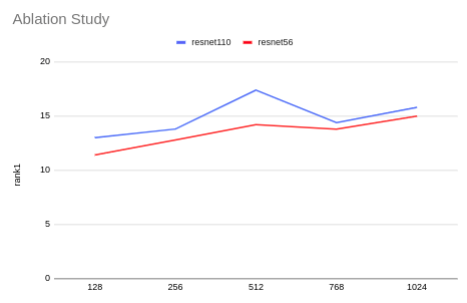
\includegraphics[scale=0.43]{img/ablation.png}
	\caption{Hasil Studi Ablasi pada \textit{Fully Connected Layer}}
	\label{fig: fclayer}
\end{figure}

Dari hasil percobaan yang dilakukan didapatkan bahwa menggunakan \textit{Fully Connected Layer} sebesar 512 mendapatkan hasil yang paling baik, dimana ketika menggunakan \textit{Fully Connected Layer} lebih dari 512 menyebabkan \textit{overfitting}. Sedangkan ketika menggunakan \textit{Fully Connected Layer} dibawah 512 tidak se-efektif menggunakan 512 layer. Gambar \ref{fig: fclayer} menunjukan grafik Rank-1 terhadap \textit{Fully Connected Layer}.

\begin{longtable}{|c|c|c|c|c|}
	\caption{Rata-rata performa semua ResNet dengan \textit{Fully Connected Layer} berbeda-beda}
	\label{tabel: 18}\\
	\hline
	\rowcolor[HTML]{C0C0C0}
	\textbf{Name} & \textbf{Rank-1} & \textbf{Rank-5} & \textbf{Rank-10} & \textbf{mAP} \\ \hline
	ResNet 56 FC 128 & 11.4\% & 36.4\% & 50\% & 15.4205\%\\ \hline
	ResNet56 FC 256 & 12.8\% & 31.8\% & 48\% & 15.71973\%\\ \hline
	ResNet 56 FC 512 & 14.2\% & 35\% & 47.8\% & 16.95365\%\\ \hline
	ResNet56 FC 768 & 13.8\% & 35.8\% & 46.8\% & 16.50338\%\\ \hline
	ResNet 56 FC 1024 & 15\% & 35.6\% & 51\% & 17.58063\%\\ \hline
	ResNet 110 FC 128 & 13\% & 35.8\% & 49\% & 15.81262\%\\ \hline
	ResNet 110 FC 256 & 13.8\% & 38.4\% & 52.8\% & 16.87966\%\\ \hline
	ResNet 110 FC 512 & 17.4\% & 38.8\% & 52.2\% & 18.87587\%\\ \hline
	ResNet 110 FC 768 & 14.4\% & 36.8\% & 48.8\% & 16.49\%\\ \hline
	ResNet 110 FC 1024 & 15.8\% & 39\% & 53.4\% & 18.0541\%\\ \hline
\end{longtable}

\begin{figure} [!htb]
	\centering
	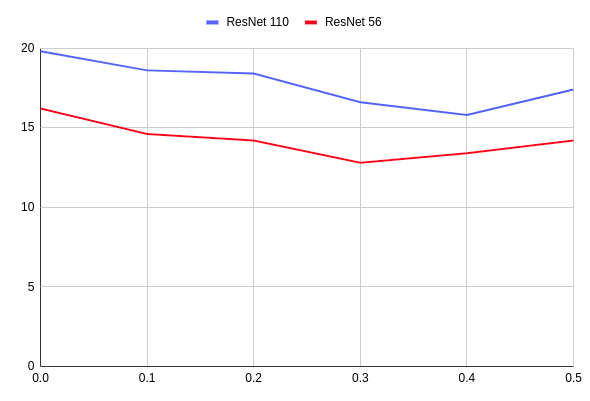
\includegraphics[scale=0.35]{img/HasilRandomErasing.png}
	\caption{Hasil Studi Ablasi pada \textit{Random Erasing}}
	\label{fig: rerasing}
\end{figure}

Sedangkan dari hasil percobaan pada \textit{Random Erasing}, didapatkan bahwa tidak menggunakan Random Erasing merupakan yang paling baik untuk model, dimana ketika menggunakan \textit{Random Erasing} performa model menurun. Sehingga ketika menggunakan Random Erasing 40\% keatas performa model menjadi tidak konsisten. Gambar \ref{fig: rerasing} menunjukan grafik Rank-1 terhadap \textit{Random Erasing}.

\section{Pengujian dengan menggunakan Ensemble}
\vspace{1ex}
Untuk meningkatkan performa dari model sendiri, dibuat sebuah ensemble dari model ResNet 56 dan ResNet 110, dimana Fully Connected layer yang digunakan sejumlah 512 layer dan tidak dilakukan Random Erasing. Selain itu dilakukan penambahan Spatial Pyramid Pooling pada ensemble dengan harapan terjadi penambahan presisi dan akurasi. Pada semua model telah dilakukan \textit{pre-training} di dataset Market 1501.

\subsection{Ensemble}
\vspace{1ex}
Pada model ini terjadi peningkatan pada Rank-1,Rank-5, Rank-10 dan mAP apabila dibandingkan dengan ResNet 110.
 
\begin{longtable}{|c|c|c|c|c|}
	\caption{Rata-rata performa ensemble }
	\label{tabel: 19}\\
	\hline
	\rowcolor[HTML]{C0C0C0}
	\textbf{No} &\textbf{Rank-1} & \textbf{Rank-5} & \textbf{Rank-10} & \textbf{mAP} \\
	\hline
	1 &24 &40 &48 &23.5601 \\
	2 &22 &40 &52 &23.8937 \\
	3 &24 &42 &60 &22.5622 \\
	4 &14 &46 &50 &18.1273 \\
	5 &26 &48 &58 &24.3952 \\
	6 &22 &44 &48 &22.6432 \\
	7 &24 &44 &50 &24.3334 \\
	8 &18 &42 &54 &21.0525 \\
	9 &14 &40 &58 &18.2236 \\
	10 &22 &38 &46 &21.7579 \\
	\hline
	\textbf{Average} & 21 & 42.4 & 52.4 &22.05491 \\
	\hline
\end{longtable}

Namun apabila dilihat dari waktu training yang dibutuhkan ensemble ini membutuhkan lebih lama dari hanya menggunakan ResNet 110.

\subsection{Ensemble + Spatial Pyramid Pooling}

\begin{longtable}{|c|c|c|c|c|}
	\caption{Rata-rata performa ensemble + Spatial Pyramid Pooling }
	\label{tabel: 20}\\
	\hline
	\rowcolor[HTML]{C0C0C0}
	\textbf{No} &\textbf{Rank-1} & \textbf{Rank-5} & \textbf{Rank-10} & \textbf{mAP} \\
	\hline
	1 &22 &44 &54 &21.425 \\
	2 &18 &44 &56 &19.6589 \\
	3 &12 &34 &48 &16.9387 \\
	4 &26 &44 &50 &23.9654 \\
	5 &16 &32 &44 &17.8318 \\
	6 &22 &48 &58 &22.1528 \\
	7 &26 &40 &52 &23.0882 \\
	8 &22 &44 &54 &21.987 \\
	9 &20 &42 &56 &21.0866 \\
	10 &18 &48 &58 &21.3644 \\
	\hline
	\textbf{Average} & 20.2 & 42 & 53 & 20.94988 \\
	\hline
\end{longtable}

Pada pengujian dengan tambahan Spatial Pyramid Pooling terjadi overfitting sehingga semua metrik evaluasi yang digunakan menurun. 

\section{Perbandingan dengan model-model lain}
\vspace{1ex}

Tabel \ref{tabel:comparison} menunjukan perbandingan performa model yang dibuat dengan model-model lain. Dari tabel tersebut dapat dilihat bahwa pada model yang dibuat Rank-1 dan Rank-5, dan Rank-10 yang didapatkan bukanlah yang terbaik.Namun pada kolom parameter dapat dilihat bahwa parameter yang dimiliki tidak sebanyak model-model lain yang pernah digunakan untuk memecahkan masalah pada dataset PKU Sketch Re-ID. Bahkan ensemble yang paling berat hanya memiliki sekitar 28.6\% parameter dari model Dense-HOG+LBP+Siamese.

\begin{longtable}{|c|c|c|c|c|}
	\caption{Perbandingan dengan model-model lain}
	\label{tabel:comparison}\\
	\hline
	\rowcolor[HTML]{C0C0C0}
			\textbf{Nama} & \textbf{Param} & \textbf{Rank-1} & \textbf{Rank-5} & \textbf{Rank-10} \\ \hline
Dense-HOG+LBP+SVM & 8.6M & 5.1\% & 16.8\% & 28.3\% \\ \hline
Triplet SN & n/a & 9\% & 26.8\% & 43.2\% \\ \hline
GN Siamese & ~14M & 28.9\% & 54\% & 62.4\%\\ \hline
Cross-Domain Adversarial & n/a & 34\% & 56.3\% & 72.5\%\\ \hline
Ensemble FC 512 & 3M & 21 \% & 42.4\% & 52.4\% \\ \hline
Ensemble SPP & 3M & 20.2\% & 42\% & 53\% \\ \hline
ResNet 110 FC 512 & 1.7M & 19.8\% & 37.4\% & 47.8\%\\ \hline
\end{longtable}


